
%(BEGIN_QUESTION)
% Copyright 2010, Tony R. Kuphaldt, released under the Creative Commons Attribution License (v 1.0)
% This means you may do almost anything with this work of mine, so long as you give me proper credit

A PLC is used to control the starting and stopping of an air compressor:

$$\includegraphics[width=15.5cm]{i03362x01.eps}$$

Identify how you could safely remove the ``cut-out'' pressure switch from this running system for testing without shutting off the compressor.

\underbar{file i03362}
%(END_QUESTION)





%(BEGIN_ANSWER)

The PLC's ``X1'' input must somehow be {\it forced} to an active state in order for the cut-out switch to be disconnected without shutting off the compressor motor.  PLC programming software provides the ability for the user to ``force'' bits in the PLC's memory for purposes just like this.

\vskip 10pt

Another issue to consider is how to safely un-wire the cut-out pressure switch when it is powered by potentially dangerous voltage (120 VAC).  The wiring for this switch would have to be provided with disconnecting terminal blocks or some other form of electrical disconnect in order for you to un-do the wire connections without contacting live conductors.

%(END_ANSWER)





%(BEGIN_NOTES)


%INDEX% Process: air compressor and receiver tank
%INDEX% Safety, shutdown system: trip testing

%(END_NOTES)

